\sec{Migration: Case Study}
\ssec{Migrating to AWS}

\begin{frame}[allowframebreaks,fragile]{Migration}

Goals
\i Evaluating the costs for a cloud/on-premises data platform
\i Fill in this table
\begin{table}[h!]
    \centering
    \begin{tabular}{ccc}
        Cost     &  On-premises & On cloud  \\\hline
        Hardware & ?            & ?         \\
        Software & ?            & ?         \\
    \end{tabular}
\end{table}
\i Real-world case study


\framebreak



\begin{figure}
    \centering
    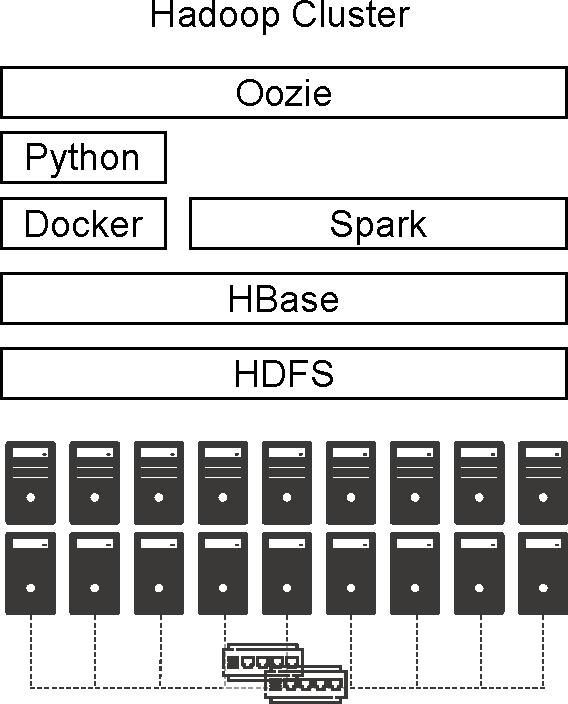
\includegraphics[scale=.5]{imgs/migration.pdf}
    \caption{On-premises (reference) architecture}
\end{figure}

\framebreak

\begin{figure}
    \centering
    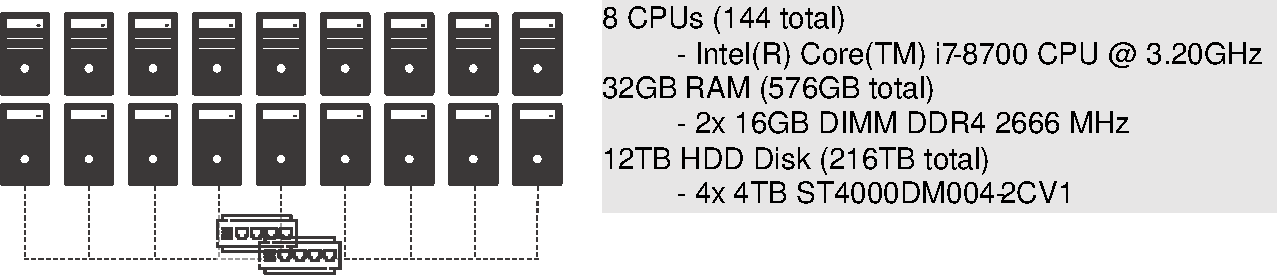
\includegraphics[scale=.5]{imgs/migration0.pdf}
    \caption{Hardware requirements}
\end{figure}

\begin{lstlisting}
lshw -short -C cpu
lshw -short -C memory
lshw -short -C disk
\end{lstlisting}

Software stack
\i Classic Hadoop stack plus Python and Docker

\framebreak

Software cost \r{(up to 2020): 0\euro{}}
\i Free Cloudera Management System
\i No software licensing (for research purpose)

Hardware cost \r{(up to Mar 05, 2021): ?}
\i \url{https://www.rect.coreto-europe.com/}

\framebreak

\begin{figure}
    \centering
    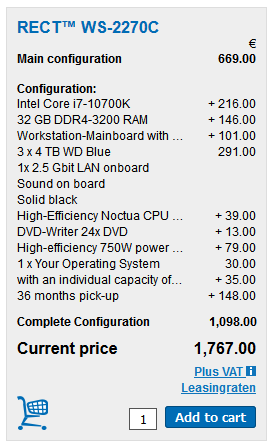
\includegraphics[scale=.5]{imgs/migration_hw_onprem.PNG}
\end{figure}

\framebreak

Software cost (up to 2020): 0\euro{}
\i Free Cloudera Management System
\i No software licensing (for research purpose)

Hardware cost (up to Mar 05, 2021): $1767\euro{} \cdot 18 = 31806\euro{}$
\i \url{https://www.rect.coreto-europe.com/}
\i Amortization over 3 years (i.e., 10602\euro{}/year)

\begin{table}[h!]
    \centering
    \footnotesize
    \begin{tabular}{ccc}
        Cost     &  On-premises  & On cloud  \\\hline
        Hardware & 10602\euro{}/year & ?         \\
        Software & 0             & ?         \\
    \end{tabular}
\end{table}

\framebreak

Software cost \r{(up to Mar 05, 2021): 10000\euro{}/year $\cdot 18$ = 180000\euro{}/year}
\i \r{Cloudera is no more free, 10K\euro{} per node}
\si {\footnotesize \url{https://www.cloudera.com/products/pricing.html#private-cloud-services}}
\si {\footnotesize \url{https://www.cloudera.com/products/pricing/product-features.html}}
\i No license for research purpose

\begin{table}[h!]
    \centering
    \footnotesize
    \begin{tabular}{ccc}
        Cost     &  On-premises            & On cloud  \\\hline
        Hardware &  10602\euro{}/year      & ?         \\
        Software & \r{180000 \euro{}/year} & ?         \\
    \end{tabular}
\end{table}

\textit{``Houston we've had a problem!''}
\i We cannot update/extend the cluster anymore

\framebreak

Moving a Hadoop cluster to the cloud (we only consider AWS)
\i AWS price calculator \url{https://calculator.aws/#/estimate}

How do we start?
\i we need architectural/application requirements
\si we already defined the hardware and the software stack
\i start with coarse tuning, identify the dominating costs first
\si is it computing, storage, or processing?
\i identify a suitable budget, implement, refine later
\si wrong refinements can do a lot of damage

\framebreak

Migrate the cluster as-is: 13500\$/month = 162000\$/year
\i 18 EC2 instances (t4g.2xlarge), 12TB EBS storage each machine
\i Still, we have no software stack configuration

\begin{figure}
    \centering
    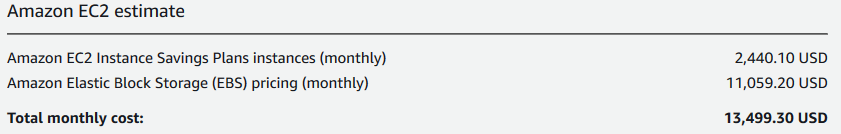
\includegraphics[scale=.5]{imgs/migration_aws_asonprem1.PNG}
\end{figure}

\begin{table}[h!]
    \centering
    \footnotesize
    \begin{tabular}{ccc}
        Cost     &  On-premises       & On cloud          \\\hline
        Hardware &  10602\euro{}/year & \r{162000\$/year} \\
        Software & 180000\euro{}/year & ?                 \\
    \end{tabular}
\end{table}

\i Also, pick the right region

\begin{figure}
    \centering
    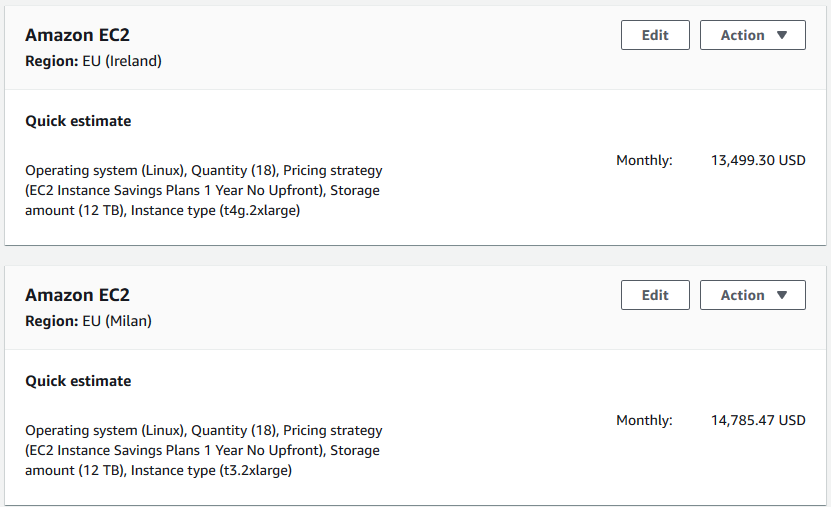
\includegraphics[scale=.5]{imgs/migration_aws_asonprem.PNG}
\end{figure}

\framebreak

It makes no sense to move the cluster as-is
\i more machines ensure better scalability but higher costs
\i let's think about some optimization
\i we need have some minimum software requirements
\si how many machines do we need at minimum?

\framebreak

\begin{figure}
    \centering
    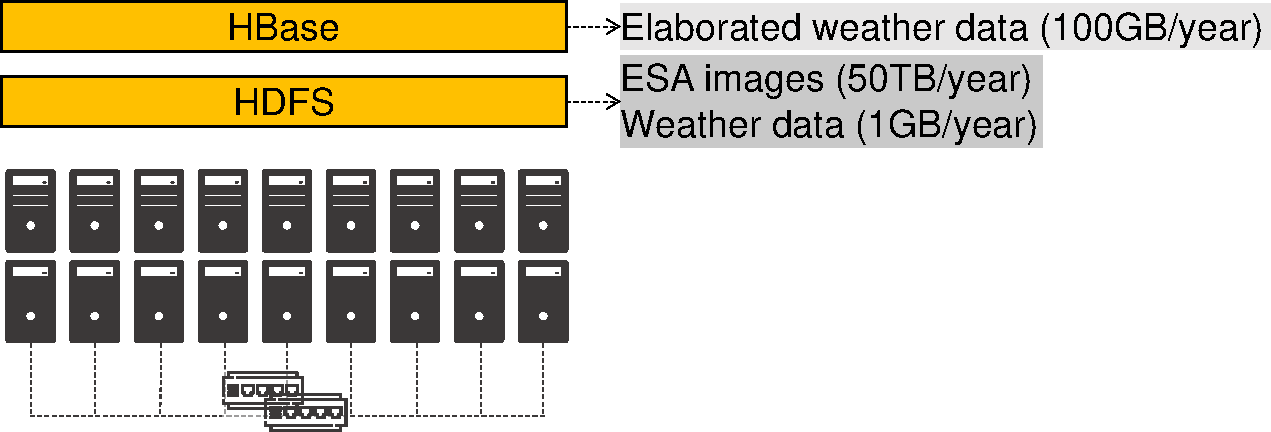
\includegraphics[scale=.5]{imgs/migration1.pdf}
    \caption{Storage}
\end{figure}

\framebreak

\textbf{HDFS}
\i How much durability do we need? (i.e., how many replicas)
\i We can think about a durability decreasing over time
\si HP1: two replicas for fresh data
\si HP2: move cold data to a glacier or delete id
\si Is it cheaper to store data or (re)process them?

\textbf{HBase} has marginal effects on the pricing ($100GB \ll 50TB$)
\i For simplicity, we can omit it (focus on the high costs)

\textbf{Overall}: 50TB storage/year

\framebreak

\begin{figure}
    \centering
    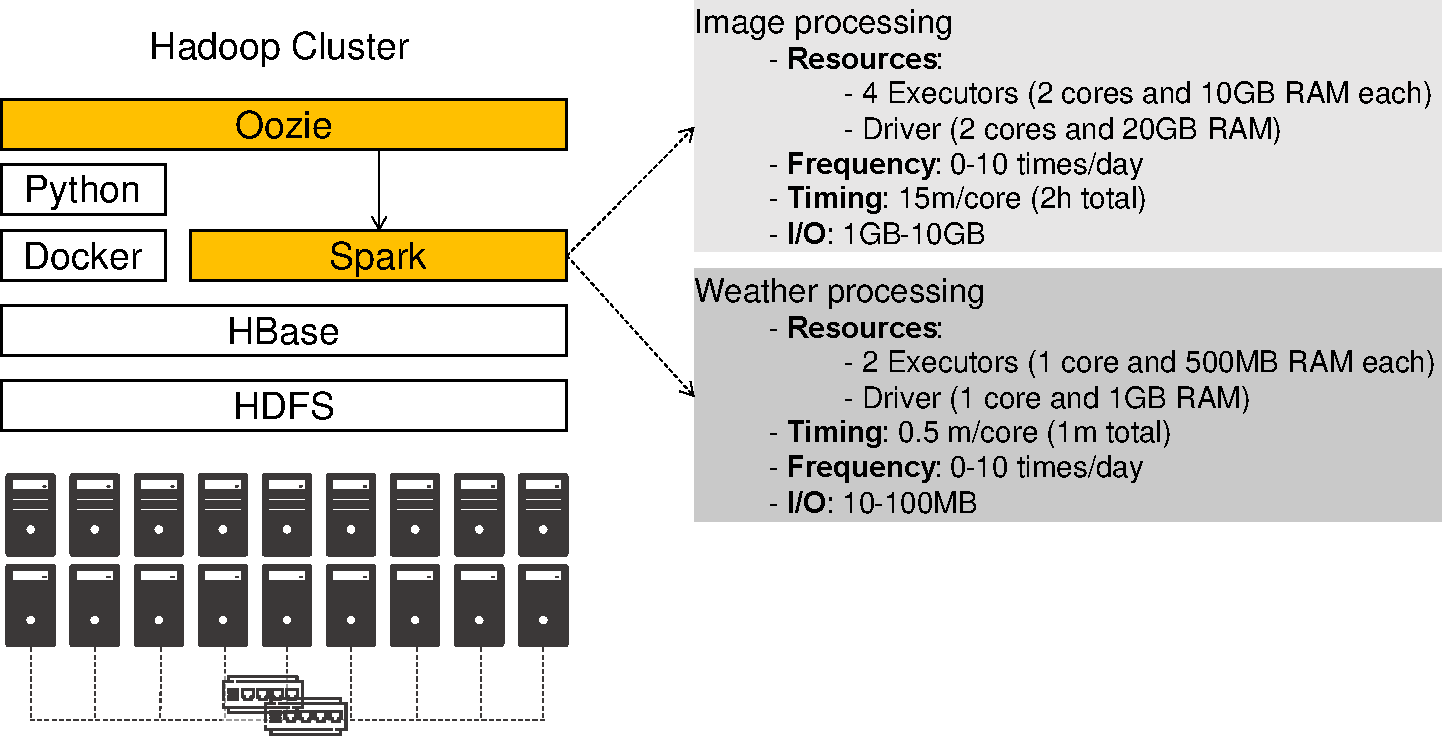
\includegraphics[scale=.5]{imgs/migration2.pdf}
    \caption{Processing}
\end{figure}

\framebreak

Processing takes place each time that ESA provides a satellite image
\i Some days no images are available
\i Some days up to 10 images are available
\i Each image is about 1GB
\i Processing produces new images with about the same same
\i Spark jobs are always executed with the same parameters 

\textbf{Image processing}
\i 4 machines, 2 cores and 10GB RAM at least

\textbf{Weather processing} is negligible, we can omit it

\framebreak

How do we proceed with the migration?

Try to achieve the smallest migration impact
\i find the most similar cloud-based solution to a Hadoop cluster
\i rethink applications when you got the know-how

Rethinking cloud-based applications (business processes) means
\i understand the application requirements of each process
\i rethink all the applications in a cluster fashion
\i much harder

\framebreak

Compare 4 machines on-premises vs on cloud

On-premises
\i 4 machines: 196\$/month = 2356\$/year
\i Cloudera requires at least 10 nodes: 100000\$/year

Migrate the cluster with minimal requirements: 1367\$/month = 16404\$/year
\i 4 EC2 instances (t4g.2xlarge), 12TB EBS storage each machine
\i Still, we have no software stack configuration

\framebreak

\begin{figure}
    \centering
    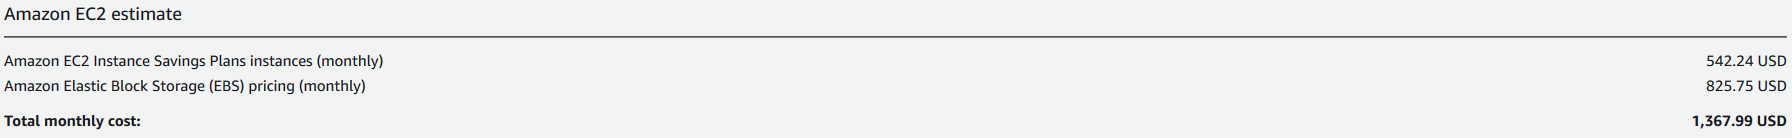
\includegraphics[scale=.5]{imgs/migration_aws_asonprem2.PNG}
\end{figure}

\begin{table}[h!]
    \centering
    \footnotesize
    \begin{tabular}{ccc}
        Cost     &  On-premises       & On cloud          \\\hline
        Hardware &  2356\euro{}/year  & \r{16404\$/year} \\
        Software & 100000\euro{}/year & ?                 \\
    \end{tabular}
\end{table}

\framebreak

Amazon EMR is the most similar service to Cloudera
\i Create/delete a cluster at need

% e (e.g., costo on demand istanza 8XL è 1.76\$, costo spot 0.5\$ ma dipende anche adlla disponibilità di availability zone---i dati non si spostano da region, è a carico nostro istanziare il cluster in una region).
\i Computational nodes (based on EC2)
\si \textit{master} node, manages the cluster (always active)
\si \textit{core} nodes, computation + data
\ssi include the HDFS demon (this cannot be turned off)
\ssi Hard to scale
\si \textit{task} nodes: core nodes without data demon
\ssi write to S3, not to HDFS
\ssi Easy to (auto)scale 
\ssi Decoupling processing and storage, we loose data locality
% (Scalare i nodi computazionali non è immediato, in quanto contengono i dati; ecco perché il disaccoppiamento è importante. MA salta il motivo della località dei dati, è vero ma EMR file system è ottimizzato, il nodo trasferisce solo i dati che necessita). 
% - console per il management
% - connettori per altri servizi AWS (S3, Dynamo DB, Code, Stream, Redshift)
% - sicurezza 
% - virtual private cloud AWS per comunicare con altri servizi o VPN per connettersi su AWS
% - MapReduce (batch), Tez (interactive), Spark (in meomory), Flin (stream)
 
\framebreak

% Worst-case (all nodes on-demand): 22K\$/year
% \i EMR service (210\$/month), pricing depends on the node number
% \i Milan Region costs 5\%/15\% more than Ireland 
% \i 1 master node, 1 core node, 4 task nodes
% \si master/core node: t5.??: ??
% \si task node: m5.xlarge, 16 GB RAM (80 in tot), 4 CPUs (20 in tot)
% \i S3 Storage (50TB, 670\$/month infrequent access)
% \si EBS costs are much higher

Migrating cluster to EMR: 14710\euro{}/year
\i \r{S3 Infrequent Access storage (50 TB per month): 640\euro{}}
\i 1 x Master EMR nodes, EC2 (m4.xlarge), Utilization (75 h/month): 4.5\euro{}
\i 1 x Core EMR nodes, EC2 (m4.xlarge), Utilization (75 h/month): 4.5\euro{}
\i 4 x Task EMR nodes, EC2 (m4.4xlarge), Utilization (75 h/month): 72\euro{}
\i 4 x EC2 on demand (task node): 174.83\euro{}
\si Storage amount (30 GB)
\si Workload (Daily, Duration of peak: 0 Hr 15 Min)
\si Instance type (m4.xlarge)
\i 2 x EC2 on demand (master and core nodes): 330\euro{}
\si Storage amount (30 GB)
\si Instance type (m4.xlarge)

\begin{table}[h!]
    \centering
    \footnotesize
    \begin{tabular}{ccc}
        Cost     &  On-premises       & On cloud                           \\\hline
        Hardware &  2356\euro{}/year  & \multirow{2}{*}{14710\euro{}/year} \\
        Software & 100000\euro{}/year &                                    \\
    \end{tabular}
\end{table}

\framebreak

Can we do better?

On-Demand Instance
\i pay for compute capacity by the hour (minimum of 60 seconds)
\i no long-term commitments

Spot Instance 
\i unused EC2 instance that is available for less than the on-demand price
\i hourly price is called a spot price
\si adjusted based on long-term supply and demand for spot instances
\si runs when capacity is available and price lower than threshold
\i when data-cetenter resources are low, spot instances are dropped
\si only suitable for batch workloads

\textit{Capacity-optimized} strategy
\i allocated instances into the most available pools
\i look at real-time capacity data, predict which are the most available
\i works well for workloads such as big data and analytics
\i works well when we have high cost of interruption 

\textit{Lowest-price} strategy
\i allocates instances in pools with lowest price at time of fulfillment


\framebreak

Migrating cluster to EMR: 13445\euro{}/year
\i S3 Infrequent Access storage (50 TB per month): 640\euro{}
\i 1 Master EMR nodes, EC2 (m4.xlarge), Utilization (75 h/month): 4.5\euro{}
\i 1 Core EMR nodes, EC2 (m4.xlarge), Utilization (75 h/month): 4.5\euro{}
\i 4 Task EMR nodes, EC2 (m4.4xlarge), Utilization (75 h/month): 72\euro{}
\r{
\i 4 x EC2 spot (task node): 69.55\euro{}
\si Storage amount (30 GB)
\si Workload (Daily, Duration of peak: 0 Hr 15 Min)
\si Instance type (m4.xlarge)
}
\i 2 x EC2 on demand (master and core nodes): 330\euro{}
\si Storage amount (30 GB)
\si Instance type (m4.xlarge)

\framebreak

\begin{table}[h!]
    \centering
    \footnotesize
    \begin{tabular}{ccc}
        Cost     &  On-premises       & On cloud                           \\\hline
        Hardware &  2356\euro{}/year  & \multirow{2}{*}{13445\euro{}/year} \\
        Software & 100000\euro{}/year &                                    \\
    \end{tabular}
\end{table}

Can we do better?
\i Pick ad-hoc cloud services
\si E.g., AWS Lambda e AWS Batch (container Docker)
\i ... to re-build the applications (food for thoughts)

\end{frame}



% Spero di aver inquadrato meglio la descrizione.

% Domande:
% - Soluzione ibrida, possiamo mantenere durability variabile in base alla freschezza del dato? Così che siamo sicuri di avere il dato nuovo, quello vecchio, se corrotto, lo buttiamo/ricomputiamo.
% - Dove manteniamo i dati? Costi e servizi diversi in base alla zona


    
 
    


% File system ha blocchi (HDFS) costa di più di storage a oggetti.

% Il traffico dati entro AWS non si paga

% Single page application (front end):
%     - Host statico direttamente in bucket S3 

% Back-end:
%     - Macchina virtual con stack web


    

